\documentclass{article}
\usepackage{amsmath,amssymb,amsthm}
\usepackage{enumerate}
\usepackage{mathtools}
\usepackage{graphicx}
\usepackage{caption}
\usepackage{bm}
\newtheorem{theorem}{Theorem}
\newtheorem{question}[theorem]{Question}
\newtheorem{answer}[theorem]{Solution}
\newcommand{\vect}[1]{\boldsymbol{\mathbf{#1}}}
\newcommand{\myvec}[1]{\ensuremath{\begin{pmatrix}#1\end{pmatrix}}}

\begin{document}
\begin{question}
	Show that the vectors $\vect{A}=\myvec{-2 \\ +1 \\ -1}$,$\vect{B}=\myvec{+2 \\ -1 \\ +1}$ and $\myvec{+1\\-3\\-5}$
form the vertices of a right angled triangle.
\end{question}
Solution. Let $\vect{A}$,$\vect{B}$  and $\vect{C}$ be given vectors such that $\vect{A} = \myvec{-2 \\ +1 \\ -1}$ \\
$\vect{B}=\myvec{+2 \\ -1 \\ +1}$ and $\vect{C}= \myvec{+1\\-3\\-5}$
Given below is the figure formed by $\vect{A}$, $\vect{B}$ and $\vect{C}$.

\begin{figure}[!htb]
	
	\centering
	
	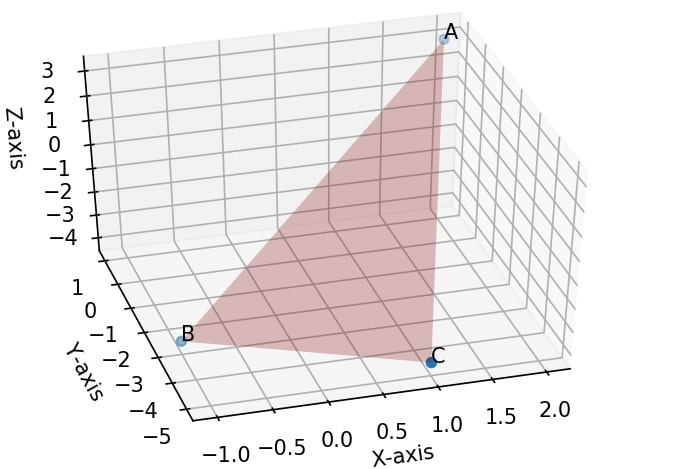
\includegraphics[width=\columnwidth]{assignment1fig-1.jpg}
	
	\caption{\label{fig1}}
	
	\label{fig:}
	
\end{figure}
Clearly, $\vect{A}\vect{B}\vect{C}$ is a triangle.
To prove, the $\triangle ABC$ is a right triangle, we need to calculate the inner product of all the below vectors and check if any one of them is 0.:
\begin{align}
	(\vect{A} -\vect{C})^T (\vect{B}-\vect{C}) = (-1 \quad+3 \quad +5) \myvec{-2 \\ +1 \\ -1}  = 00 \\
	(\vect{A} -\vect{B})^T (\vect{C}-\vect{B})
	 = (+1 \quad +2 \quad +6) \myvec{+2 \\ -1 \\ +1} = 06 \\
    (\vect{B} -\vect{A})^T (\vect{C}-\vect{A}) = (-1\quad-2 \quad-6) \myvec{+1\\-3\\-5} = 35 
\end{align}
Clearly, from ($1$) we can see that $\triangle$ABC is right angled at C.
\end{document}
